\documentclass[
	12pt,
	a4paper,
	BCOR10mm,
	%chapterprefix,
	DIV14,
	headsepline,
	%twoside,
	%openright
]{scrreprt}

\KOMAoptions{
	listof=totoc,
	bibliography=totoc,
	index=totoc
}

\usepackage[T1]{fontenc}
\usepackage[utf8]{inputenc}

\usepackage{lmodern}

\usepackage[ngerman,english]{babel}

\usepackage[toc]{appendix}
\usepackage{eurosym}
\usepackage{fancyhdr}
\usepackage{graphicx}
\usepackage[htt]{hyphenat}
\usepackage{listings}
\usepackage{microtype}
\usepackage[list=true,hypcap=true]{subcaption}
\usepackage{units}

\usepackage{varioref}
\usepackage[hidelinks]{hyperref}
\usepackage[capitalise,noabbrev]{cleveref}

\usepackage{wrapfig}

\renewcommand*{\thefootnote}{\fnsymbol{footnote}}

\lstset{
	basicstyle=\ttfamily,
	frame=single,
	numbers=left,
	language=C,
	breaklines=true,
	breakatwhitespace=true,
	postbreak=\hbox{$\hookrightarrow$ },
	showstringspaces=false,
	tabsize=4,
	captionpos=b,
	morekeywords={gboolean,gpointer,gconstpointer,gchar,guchar,gint,guint,gshort,gushort,glong,gulong,gint8,guint8,gint16,guint16,gint32,guint32,gint64,guint64,gfloat,gdouble,gsize,gssize,goffset,gintptr,guintptr,int8_t,uint8_t,int16_t,uint16_t,int32_t,uint32_t,int64_t,uint64_t,size_t,ssize_t,off_t,intptr_t,uintptr_t,mode_t}
}

\makeatletter
\renewcommand*{\lstlistlistingname}{List of Listings}
\makeatother

\begin{document}

\begin{titlepage}
	\begin{center}
		{\titlefont\huge SCIL - Scientific Compression Interface Library\par}

		\bigskip
		\bigskip

		{\Large Project Report\par}

		\bigskip
		\bigskip

		{\large Arbeitsbereich Wissenschaftliches Rechnen\\
		Fachbereich Informatik\\
		Fakultät für Mathematik, Informatik und Naturwissenschaften\\
		Universität Hamburg\par}
	\end{center}

	\vfill

	{\large\begin{tabular}{ll}
		Vorgelegt von:  & Armin Schaare \\
		E-Mail-Adresse: & \href{mailto:adresse@email.de}{3schaare@informatik.uni-hamburg.de} \\
		Matrikelnummer: & 6423624 \\
		Studiengang:    & Informatik \\
		\\
		Hamburg, den 05.04.2016
	\end{tabular}\par}
\end{titlepage}

\chapter*{Abstract}

\thispagestyle{empty}


This report presents the developement process, design and current state of SCIL
- the Scientific Compression Interface Library. After a short introduction to
compression in general and a documentation on design and implementation
of SCIL follows.

\tableofcontents

\chapter{Introduction}
\label{Introduction}

\section{Data Compression}

\bigskip

Data compression is the encoding of information to reduce its bit size while
still adequately representing the original information [citation needed].
Thus data compression can be used to maximize effective storage capacities of
given hardware as well as reducing the load on bandwidth limited networks.
Large amounts of data generated in scientific as well as commercial research
environments and limited budgets for data storage and processing give rise to
the need of better and faster compression techniques. The Large Hadron Collider
at CERN for example is generating 600 Terabyte of collision event data per
second. Unable to process such volumes of data, scientists filter out the most
promising data, generally leaving 100 - 200 Megabyte per second of 'interesting'
information which needs to be stored [citation needed]. Another example where
data compression is very applicable is climate research. In particle collision
data few interesting events are of concern, whereas for climate research it is
beneficial to record and process as much available data as possible
[citation needed]. In any case, compression leads to more data being stored and
processed, contibuting to better and faster research.

\begin{wrapfigure}{l}{0.6\textwidth}
	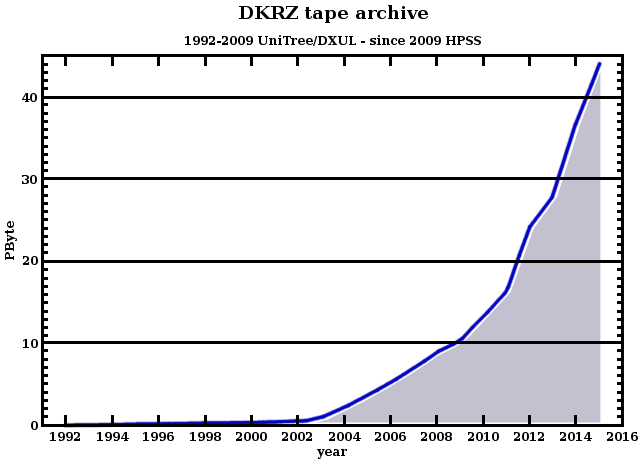
\includegraphics[width=0.9\linewidth]{DKRZ_data_growth.png}
	\caption{DKRZ data growth redrawn\\ citation needed}
	\label{fig:dkrz}
\end{wrapfigure}

\cref{fig:dkrz} illustrates the increasing data usage at the German Climate
Computing Center in Hamburg (DKRZ). Until now data compression at the DKRZ
already has been put to practise but "storage capacity does not grow as fast as
computation power" [citation needed]. Therefore optimizations regarding data
reduction are a reasonable method to minimize the need of upscaling existing
data archives.
\clearpage

\section{SCIL}

To further exploit the potential of lossy and lossless compression in research,
SCIL is being developed. SCIL is the Scientific Compression Interface
Library for the programming language C. Having conventional and specifically
developed compression algorithms integrated, it is able to compress data in
a variety of ways. After calling the program 'scil-config'\footnote{Not yet implemented}
to configure SCIL for the running platform, each compression can be customized
by providing parameters such as:

\bigskip

\begin{itemize}
	\item Absolute/Relative error tolerance
	\item Performance of compression in MB/s
	\item Dimensional layout of the data
\end{itemize}

\bigskip

Based on these parameters, the platform dependent configuration and the
characteristics of the data itself, SCIL will automatically choose the best
fitting compression algorithm at disposal\footnotemark[\value{footnote}].\par

\setcounter{footnote}{0}

\chapter{Design}
\label{Design}

\textit{%
In this chapter, ...
}

\bigskip

Lorem ipsum dolor sit amet, consetetur sadipscing elitr, sed diam nonumy eirmod tempor invidunt ut labore et dolore magna aliquyam erat, sed diam voluptua.
At vero eos et accusam et justo duo dolores et ea rebum.
Stet clita kasd gubergren, no sea takimata sanctus est Lorem ipsum dolor sit amet (see \cref{lst:listing}).

\begin{lstlisting}[caption=Example listing, label={lst:listing}]
void print (void)
{
	int i;

	for (i = 0; i < 10; i++)
	{
		printf("Hello World!\n");
	}
}
\end{lstlisting}

\chapter{Conclusion}
\label{Conclusion}

Lorem ipsum dolor sit amet, consetetur sadipscing elitr, sed diam nonumy eirmod tempor invidunt ut labore et dolore magna aliquyam erat, sed diam voluptua.
At vero eos et accusam et justo duo dolores et ea rebum.
Stet clita kasd gubergren, no sea takimata sanctus est Lorem ipsum dolor sit amet.

\bibliographystyle{alpha}
\bibliography{literatur}

\appendix
\appendixpage

\chapter{Chapter}

Lorem ipsum dolor sit amet, consetetur sadipscing elitr, sed diam nonumy eirmod tempor invidunt ut labore et dolore magna aliquyam erat, sed diam voluptua.
At vero eos et accusam et justo duo dolores et ea rebum.
Stet clita kasd gubergren, no sea takimata sanctus est Lorem ipsum dolor sit amet.

\listoffigures

\lstlistoflistings

\listoftables

\chapter*{}

\thispagestyle{empty}

\section*{Eidesstattliche Versicherung}

\begin{otherlanguage}{ngerman}
Hiermit versichere ich an Eides statt, dass ich die vorliegende Arbeit im Studiengang XXX selbstständig verfasst und keine anderen als die angegebenen Hilfsmittel -- insbesondere keine im Quellenverzeichnis nicht benannten Internet-Quellen -- benutzt habe.
Alle Stellen, die wörtlich oder sinngemäß aus Veröffentlichungen entnommen wurden, sind als solche kenntlich gemacht.
Ich versichere weiterhin, dass ich die Arbeit vorher nicht in einem anderen Prüfungsverfahren eingereicht habe und die eingereichte schriftliche Fassung der auf dem elektronischen Speichermedium entspricht.

\bigskip

\noindent
Ich bin damit einverstanden, dass meine Abschlussarbeit in den Bestand der Fachbereichsbibliothek eingestellt wird.
\end{otherlanguage}

\bigskip
\bigskip
\bigskip

\begin{center}
\begin{tabular}{ll}
	\rule{0.35\textwidth}{0.4pt} & \rule{0.55\textwidth}{0.4pt} \\
	Ort, Datum & Unterschrift
\end{tabular}
\end{center}

\end{document}
